%% LaTeX2e class for student theses
%% sections/main/1_fundamentals.tex
%%
%% Karlsruhe University of Applied Sciences
%% Faculty of Computer Science and Business Information Systems
%%
%% --------------------------------------------------------
%% | Derived from sdqthesis by Erik Burger burger@kit.edu |
%% --------------------------------------------------------


\chapter{Fundamentals}
\label{ch:Fundamentals}

The subsequent chapter provides a fundamental understanding of the concepts and general conditions, that apply in the sector of \acrshort{emobility}, and therefore are omnipresent in most of the described scenarios later on.
First of all, Section \ref{ch:Fundamentals:sec:Electric Mobility} gives a general review of \acrshort{emobility}, like the involved actors and their systems. Furthermore, existing standards for depicting the communication between these actors and systems and a brief introduction to smart charging and its variations follow.
Additionally, the subsequent Section \ref{ch:Fundamentals:sec:Reservation Systems} illustrates the basic functionality of a reservation system itself, its use cases, and a differentiation between common types of reservation systems.
Lastly, the Section \ref{ch:Fundamentals:sec:Data Exchange} lists important communication protocols and data exchange formats used in the respective standards described in \ref{ch:Fundamentals:sec:Electric Mobility:ssec:Relevant Standards}.

\section{Electric Mobility}
\label{ch:Fundamentals:sec:Electric Mobility}

The term \acrshort{emobility} generally refers to the use of \acrfull{ev} and other electric--powered transportation options as an alternative to conventional vehicles that are powered by an \acrfull{ice}. 
As a crucial element of the worldwide initiative to counter climate change and achieve sustainable transport solutions, it aims to reduce greenhouse gas emissions, lower dependence on fossil fuels and mitigate the environmental impact of transportation \cite{kathiresh_e-mobility_2022}.
To achieve this objective, \acrshort{emobility} depends on the expansion of \acrshortpl{ev} as a common means of transport and a denser cluster of \acrshortpl{cs}.
Apart from the focus on vehicles primarily addressing personal transportation, this term could also be applied in the context of freight transport, which demands much higher capacities in terms of the power required by such vehicles.
Within this research and the following chapters, only \acrshortpl{bev} used for personal transportation in the form of cars or smaller vans are considered as the respective audience.

\subsection{Electric Vehicles}
\label{ch:Fundamentals:sec:Electric Mobility:Electric Vehicles}

As already mentioned in Section \ref{ch:Fundamentals:sec:Electric Mobility}, \acrshortpl{ev} are a fundamental cornerstone of \acrshort{emobility}. Primarily, an \acrshort{ev} refers to a car that is powered by only one or more electric engines drawing energy from onboard batteries or similar energy sources. 
Besides \acrfullpl{bev}, which are purely powered by electricity, further invariants like \acrfullpl{phev} or \acrfullpl{hev} exist. In comparison to the aforementioned \acrshortpl{bev}, \acrshortpl{phev} combine the power of an electric motor with the reliance offered by an internal combustion engine.
This allows the driver to cover shorter distances solely relying on the internal battery, and use the petrol engine during longer trips or when charging is unavailable. Moreover, \acrshortpl{phev} have the capability of recharging the battery while on the move.
Therefore, brake resistance is employed to convert the power generated into electricity, feeding it directly back into the battery.
\acrshortpl{hev} closely resemble \acrshortpl{phev} as they have access to both power sources. However, unlike a \acrshort{phev}, \acrshortpl{hev} do not have the possibility to be plugged in for charging \cite{kathiresh_e-mobility_2022}.

\begin{figure}[h]
    \centering
    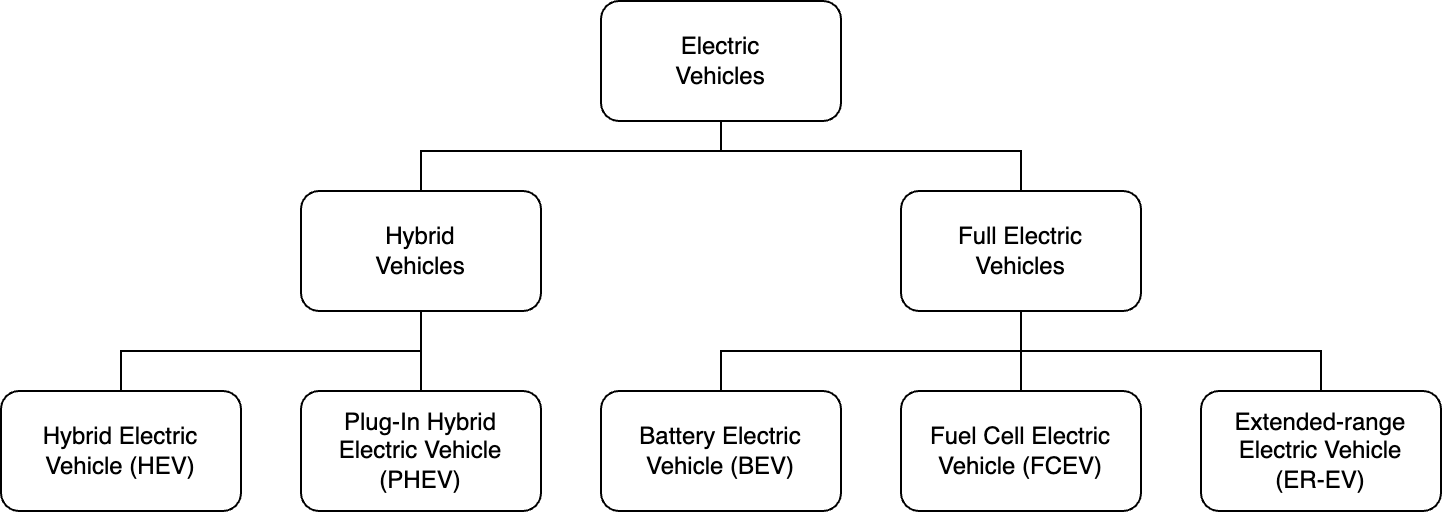
\includegraphics[width=\textwidth]{resources/images/main/1_fundamentals/ElectricVehicleTypes.png}
    \caption{Classification approach for different \acrshort{ev} types based on \cite{acharige_review_2023}.}
    \label{fig:ev-classification}
\end{figure}

\subsection{Charging Infrastructure}
\label{ch:Fundamentals:sec:Electric Mobility:ssec:Charging Infrastructure}

To facilitate the growing number of \acrshortpl{ev}, a crucial aspect is the establishment of a broad charging infrastructure comprising multiple \acrshortpl{cs}. As highlighted in \cite{gnann_fast_2018}, the requirements for charging infrastructure are highly variable, depending on the battery capacity and charging rate, which is predicted to increase in the future.
In order to satisfy the various power requirements and to cover the wide range of vehicles and used batteries, a heterogeneous range of \acrshortpl{cs} exists.
From stations providing so--called slow charging with a power supply up to 22 kW, more advanced technologies allow fast charging \acrshortpl{cs} for power requirements above this certain range. \\
\noindent For a better understanding of the different scenarios in which a \acrshort{cs} could be used for charging, this work divides the infrastructure and the corresponding stations into three different groups. 
These groups, classified according to accessibility level for the \acrshortpl{evu}, are presented in Table \ref{tab:cs-accessibility-levels} alongside their user restrictions, the associated locations, and most commonly used charger levels:

\begingroup
\setlength{\tabcolsep}{10pt} % Default value: 6pt
\renewcommand{\arraystretch}{1.5} % Default value: 1
\begin{table}[h]
\centering
\caption{Differentiation of accessibility in case of charging opportunities based on \cite{kathiresh_e-mobility_2022},\cite[18-19]{linnemann_elektromobilitat_2020}.}
    \begin{tabular}{c|c|m{5.5cm}|c}
    Accessibility & Restrictions & Location & Charging Level \\ \hline
    Public & No & fleets, highway, distribution centers & 3 \\
    Semi--Public & Yes & workplace, hotels & 2 \\
    Private & Yes & private households & 1 
    \end{tabular}
\label{tab:cs-accessibility-levels}
\end{table}
\endgroup

\newpage

\noindent Alongside the separation according to the accessibility level, a differentiation based on classes of \acrfullpl{cs} is possible. For a detailed illustration of the dependencies and relationships between the different classes, see Figure~\ref{fig:charging-station-classification} below. 

\begin{figure}[h]
\centering
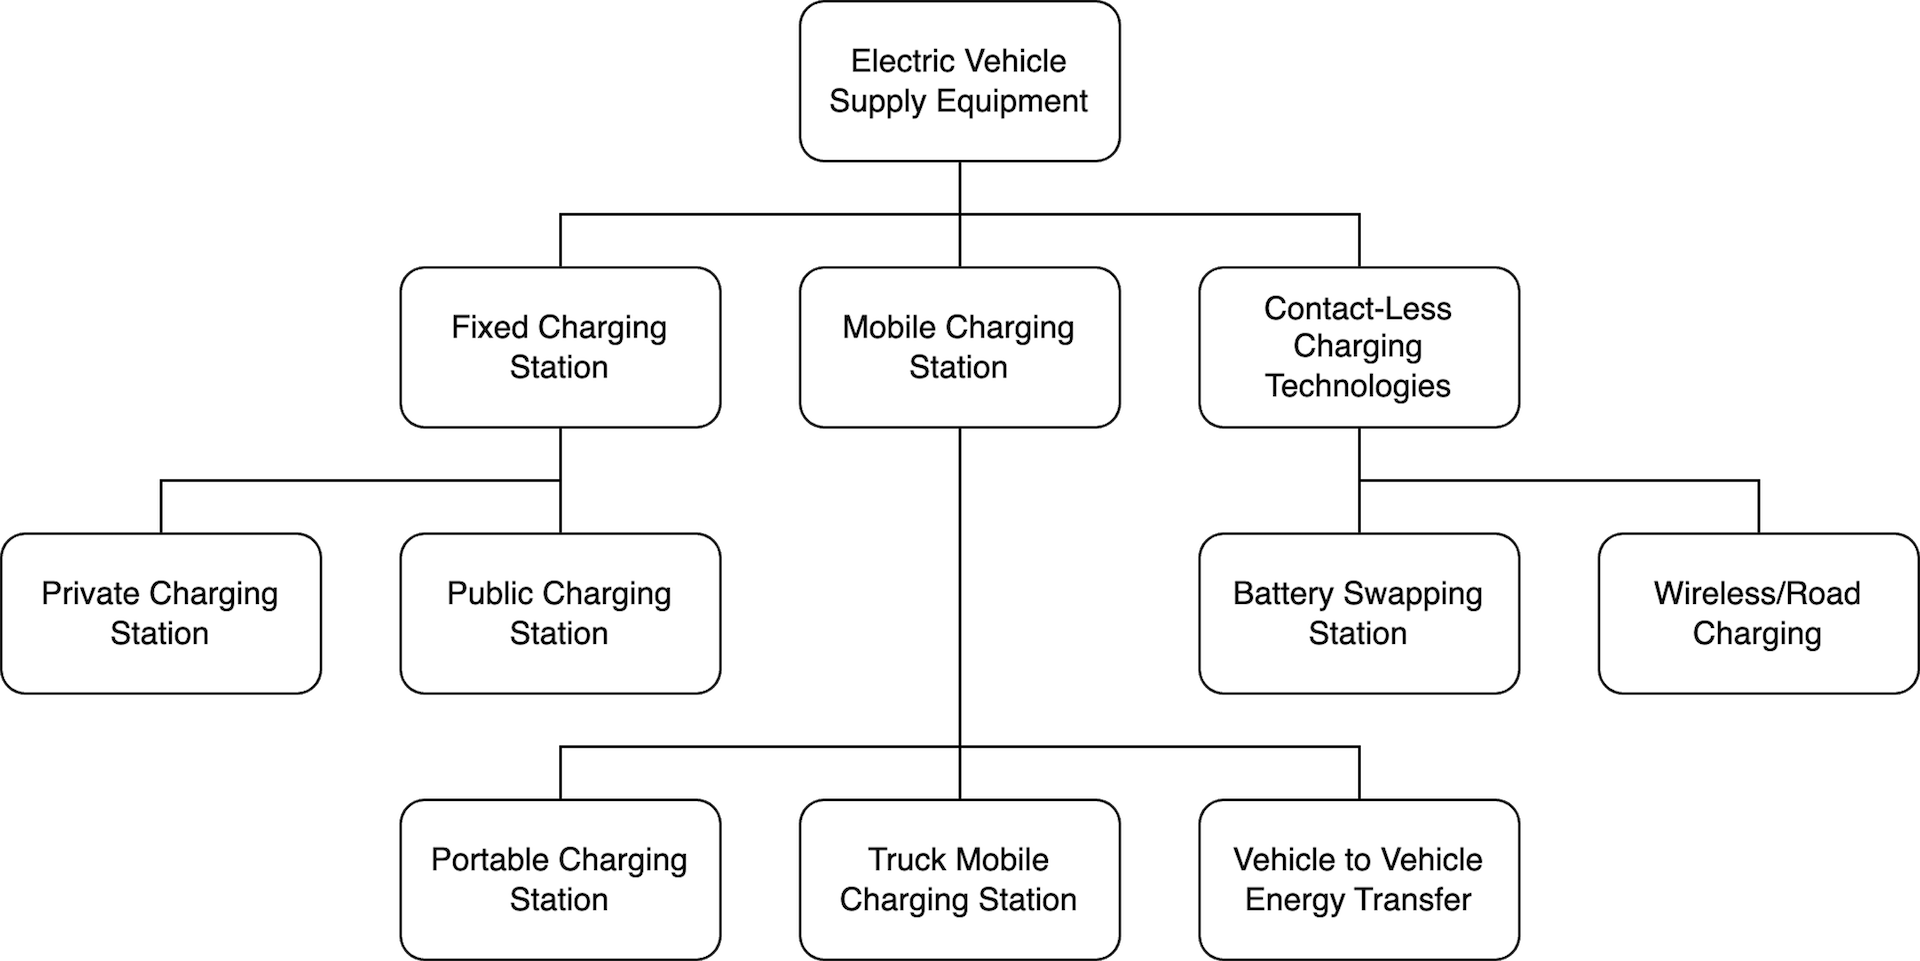
\includegraphics[width=\textwidth]{resources/images/main/1_fundamentals/ChargingStationClassification.png}
\caption{Classification for different types of \acrshortpl{cs} based on \cite{afshar_literature_2020}.}
\label{fig:charging-station-classification}
\end{figure}

\noindent To provide a more detailed view on the infrastructure and the hardware used for charging, also referred to as \acrfull{evse}, all components and systems necessary to supply electric power from the grid to the battery of an \acrfull{ev} are explained afterwards.
Beginning with the \textbf{\acrfull{cs}} itself, as physical power unit the \acrshort{ev} is connected to. As mentioned above, \acrshortpl{cs} can vary in size and complexity, ranging from small wall--mounted units designed for home use to more extensive public \acrshortpl{cs} found in parking lots, shopping centers or along highways. 
To establish a connection between grid, \acrshort{cs} and car, a \textbf{Connector or Charging Cable} is needed. It contains plugs on both ends, which are connecting to the vehicle's charging port and to the \acrshortpl{cs} outlet. 
As an integral part of the \acrshort{evse}, the \textbf{\acrshort{pms}} regulates the flow of electricity from the grid to the vehicle's battery. It ensures safe and efficient charging, managing the power level based on the vehicle's battery capacity and the grid's capacity.
Allowing the communication between the \acrshort{ev}, the \acrfull{cs}, and the grid, a \textbf{\acrshort{cms}} is used as a backend. It allows data exchange regarding charging status, electricity prices, user authentication, and other relevant information.
In the case of public \acrshortpl{cs}, a payment and authentication system is usually integrated into the \acrshort{evse}. This system verifies the user's identity, authorizes the charging session, and processes payment for the electricity consumed.
On top of the described components, various safety features are integrated to protect users, the vehicle, and the surrounding environment. Including features such as ground fault protection, over--current protection, temperature monitoring, and emergency shut--off capabilities~\cite{littlefuse_designing_2020}.
\noindent To meet the wide range of existing \acrshortpl{ev} and their individual power requirements, different categories of chargers have been established based on the power level provided. This work lists the most notable categories, along with their specifications and typical usage, in Table~\ref{tab:ev-charging-levels}. 

\begingroup
\setlength{\tabcolsep}{10pt} % Default value: 6pt
\renewcommand{\arraystretch}{1.5} % Default value: 1
\begin{table}[h]
    \centering
    \caption{Listing of different \acrshort{ev} charging levels based on \cite{acharige_review_2023}.}
    \begin{tabular}{c|c|m{6.5cm}}
        Charging Level & Charging Power & Use Case \\ \hline
         1 & 1.44 kW - 1.9 kW & Typically the slowest charging option and suitable for overnight charging at home \\
         2 & 3.1 kW - 19.2 kW & Provides faster charging compared to Level 1 and is commonly used for home charging setups and public charging stations \\
         3 & 20 kW - 350 kW & Fast charging operates at a higher voltage, directly charging the vehicle's battery with direct current power. Commonly used in public fast--charging stations.\\
         \acrshort{xfc} & > 350 kW & Ultra--fast charging provides the fastest charging option. Commonly used in commercial settings.
    \end{tabular}
    \label{tab:ev-charging-levels}
\end{table}
\endgroup

\newpage

\subsection{Battery Technology}
\label{ch:Fundamentals:sec:Electric Mobility:ssec:Battery Technology}

For storing the required energy, \acrshortpl{ev} rely on their built--in batteries. As key components inside an \acrshort{ev}, they have to handle high energy capacity and high power, within limited weight and space to affordable prices.
Therefore, most manufacturers use Lithium--ion batteries in their cars nowadays. 
Alternatives such as \textit{Lead Acid} and \textit{Nickel--based} batteries usually have lower durability compared to lithium--based batteries due to their shorter lifespan and subsequent inadequate performance in extreme weather or higher discharge rates \cite{acharige_review_2023}.
Generally, the advances in this technology leading to an increase in the range of the \acrshortpl{ev} and a reduction in the charging time, combined with cost effectiveness, are an essential part of the transition from cars using \acrshort{ice} to purely \acrshort{ev}.

\subsection{Relevant Standards}
\label{ch:Fundamentals:sec:Electric Mobility:ssec:Relevant Standards}

To establish a comprehensive interface for information exchange between \acrshortpl{cs}, \acrshortpl{ev}, and their users, various organizations, initiatives and the industry have established several standards for communication between the single actors in this particular environment.
Aside from the \acrfull{ocpp} \cite{noauthor_ocpp_nodate}, a communication protocol, developed by the \acrfull{oca} \cite{noauthor_open_nodate}, other protocols and specifications exist, covering different aspects and scenarios relevant during or before the charging process.
In addition to the previously mentioned \acrshort{ocpp}, further standards relevant to this work are listed and explained below.

\subsubsection{Open Charge Point Protocol}
\label{ch:Fundamentals:sec:Electric Mobility:ssec:Relevant Standards:sssec:OCPP}

The \acrfull{ocpp} outlines an open industry--standard communication protocol, used especially in charging infrastructure for \acrshortpl{ev}. Proposed by the ElaadNL foundation as an open protocol to support the communication between \acrshort{cs} and the related backend services, the ownership was transferred to \acrshort{oca} in 2014 \cite{garofalaki_electric_2022}.
In general, the \acrshort{ocpp} is designed to provide interoperability and seamless integration between different \acrshort{cs} vendors and network operators, ensuring that \acrshort{ev} drivers can charge their vehicles at any compatible \acrshort{cs}.
Therefore, it is maintained by the \acrfull{oca}, a consortium of \acrshort{ev} charging infrastructure stakeholders, as an open protocol and not proprietary to any specific manufacturer or organization. 
Ensuring that the \acrshort{ocpp} remains a collaborative and evolving standard \cite{noauthor_ocpp_nodate}. \\
From an architectural point of view, the protocol could be described in the form of a client/server architecture. The \acrshort{evse} in this model acts as the client, while the \acrshort{csms} serves as the server. 
The server responds to the client's requests and manages the charging processes accordingly. This request--response model, where the client sends requests to the server, and the server responds with the appropriate information or action enables real--time communication between the \acrfull{cs} and the connected \acrfull{cms}.
As an interface for communication, two different types of protocols are used. On the one side, the WebSocket protocol, described in \ref{ch:Fundamentals:sec:Data Exchange:ssec:WebSocket}, for bidirectional communication, providing a persistent connection between the \acrshort{evse} and the \acrshort{cms} and allowing a faster and more efficient data exchange. On the other side, \acrfull{soap}, as described in \ref{ch:Fundamentals:sec:Data Exchange:ssec:SOAP}, is suitable for the implementation of one--way communication between the respective entities.
To differentiate between particular feature sets, the \acrshort{ocpp} is versioned. 
The versions are presented as floating point numbers, which increase with major or minor releases within the nomenclature, such as \acrshort{ocpp} 1.6 and \acrshort{ocpp} 2.0. Representing the latest versions of the protocol, which are widely used in current implementations. \\ \\
\noindent For the communication between \acrshort{cs}, \acrshort{csms} and the \acrshort{evu}, the \acrshort{ocpp} protocol relies on so called operations. Each of these operations describes a set of instructions, which are necessary to fulfill, to successfully complete the underlying process.
According to the required operations used in the context of this work, a subset of operations are selected, which are elucidated in the following list. 
The wording and the explanations are based on the standard documentation for the \acrshort{ocpp} version 1.6 \cite{noauthor_ocpp_nodate}:

\begin{description}
    \item[Authorize] Before starting a charging session, the \acrshort{evu} \acrfull{rfid} card or other identification is sent to the central system for authorization. The \acrshort{cms} checks the driver's credentials and responds with an authorization status.
    \item[Start Transaction] After successful authorization, the \acrshort{cms} sends a start transaction request to initiate the charging process. The \acrshort{cs} acknowledges the request, and the charging session begins.
    \item[Status Notification] The \acrshort{cs} may send status notifications to the \acrshort{cms} to update the current state of the \acrshort{cs}, such as \verb|Available|, \verb|Charging|, \verb|Reserved|, or \verb|Faulted|.
    \item[ReserveNow] In case a user needs an available connector on a \acrshort{cs}, he could send a \textit{ReserveNow} request via the \acrshort{cms} to the \acrshort{cs}, which reserves one specific or at least one connector on the station for a specified duration. The according connector in case of successful reservation changes from status \verb|Available| to \verb|Reserved|.
    As a result, only the user assigned to the deposited \acrshort{rfid} card is able to start charging at the specified connector or the superior \acrshort{cs}.
    \item[Cancel Reservation] For canceling the created reservation the user has the ability to manually send a request with the assigned reservation \acrshort{id} to the \acrshort{cms}, to free the connector again. Otherwise, the \acrshort{cs} will notify the \acrshort{cms}, if the reservation reaches its expiry limit.
\end{description}

\subsubsection{Open Charge Point Interface}
\label{ch:Fundamentals:sec:Electric Mobility:ssec:Relevant Standards:sssec:OCPI}

\acrfull{ocpi} is a standardized, open protocol facilitating communication and supporting interoperability between different charging network operators, which provides \acrshort{ev} drivers with access to charging infrastructure from multiple providers. This is achieved by utilizing a harmonized approach. 
Alongside \acrshort{ocpi}, other proposals regarding the development of cross--border \acrshort{ev} travel, also known as \textit{e--roaming}, exist. 
The most prominent ones are \acrfull{oicp}, \acrfull{ochp} and \acrfull{emip} \cite{ferwerda_advancing_2018}. 
In contrast to the \acrshort{ocpi}, they are all developed by proprietary institutions and integrated inside their offerings providing dedicated roaming platforms. 
Thus, no way is provided to allow compatibility, making the \acrshort{ocpi} standard more suitable in the case of openness and interoperability. \\
\noindent In case of available features, \acrshort{ocpi} provides defined endpoints, used for communication between \acrshort{cs}, \acrshortpl{cms}, \acrshortpl{emsp} and \acrshortpl{cpo}. These endpoints include functionalities such as location discovery, charge point data, authorization, charging sessions, and error handling. 
For integrating \acrshort{ocpi} into existing software systems it is heavily based on the paradigm of \acrfull{rest}. This allows communication via standard HTTP methods utilizing \acrfull{json} as a data format for transmitting information. 

\noindent The listing below provides a short overview of available features and functionalities provided by \acrshort{ocpi} \cite{noauthor_open_2021}:

\begin{description}
    \item[Location Discovery] Charging networks can exchange information about available charging locations, providing details such as location coordinates, \acrshort{cs} types, and status.
    \item[Charge Point Data] Access to data on \acrshort{cs}, including details on availability, status, and pricing, is possible through \acrshort{ocpi}.
    \item[Charging Sessions] \acrshort{ocpi} supports real--time information about ongoing charging sessions, including start time, energy consumed, and current charging status.
    \item[Authorization and Authentication] In combination with their respective \acrshort{cpo} accounts or other authentication methods \acrshortpl{evu} are able to authenticate themselves to access charging services.
    \item[Remote Start/Stop Charging Sessions] To initiate charging sessions, \acrshortpl{evu} are capable of remotely starting and stopping their current charging sessions. This allows the driver to initiate charging sessions via their mobile apps or other remote means.
    \item[Tariff Information] Charging networks can share pricing and tariff information, providing transparency to \acrshortpl{evu} about the cost of charging at different locations.
\end{description}

\subsubsection{ISO 15118}
\label{ch:Fundamentals:sec:Electric Mobility:ssec:Relevant Standards:sssec:ISO 15118}

To meet the demands of \acrshortpl{evu} and address the problems of lack of standardization in charging infrastructure interoperability and information exchange between grid \acrshort{evse}, \acrshort{ev} and \acrshort{evu}, Daimler and RWE started a collaboration in September 2009 to enable Smart Charge Communication.
Until its initial release as the standard for Plug--n--Charge connections in June 2014, further progress towards the standardization of charging infrastructure communication was carried out \cite{heinrich_iso_2017}.
Nowadays, this standard consists of multiple parts. From the analysis of the underlying use cases to a description of requirements for the communication over the different \acrshort{osi} layers, it describes \acrshort{poi}--data, the \acrshort{cs} availability, payment, communication standards as well as the \textit{Plug \& Charge} or \textit{e--Roaming} approach \cite{brosi_methode_2019}. 
However, the required level of data granularity or quality is not specified \cite{linnemann_elektromobilitat_2020}. Considering these gaps that still exist in the \acrshort{iso} 15118, it is far from being complete and requires further development and adaptation.

\subsection{Smart Charging}
\label{ch:Fundamentals:sec:Electric Mobility:ssec:Smart Charging}

The concept of smart charging or intelligent charging is a systematic approach that optimizes the charging process of \acrshortpl{ev} to be more efficient, cost-effective, and environmentally friendly using information and communication technologies. 
Therefore, the subsequent calculations consider factors such as electricity demand, grid capacity, availability of renewable energy, and individual user preferences to allow for optimizations in the user's decision--making \cite{deb_smart_2022}.
One of the primary goals of this methodology is to balance the demand on the underlying grid, affected by charging large numbers of \acrshortpl{ev} simultaneously \cite{daina_electric_2017}. Especially during peak hours increased electricity costs or potential blackouts could result. 
In order to mitigate these situations, smart charging takes the current load of the grid into account and adjusts the possible charging rates based on the given constraints to prevent overloading the grid and optimizing the use of available energy \cite{garcia-villalobos_plug-electric_2014}. 
Compared to the unidirectional charging method originally known as \acrfull{v1g}, the approach of \acrfull{v2g} enables smart charging systems to charge bidirectionally between the \acrshortpl{ev} battery and the grid \cite[199]{kathiresh_e-mobility_2022}. Allowing \acrshortpl{ev} with sufficient battery capacity to return energy to the grid during times of high demand and turning them into mobile energy storage units to enhance grid stability and resiliency.
To offer all these functions, smart charging relies on data connectivity and communication between the single \acrshortpl{cs}, the \acrshortpl{ev}, and the underlying grid, which makes it vulnerable to malign third--party entities as well. On the other side, these factors can contribute to better grid management overall, giving grid operators insight into electricity demand patterns and enabling them to plan grid upgrades accordingly.

\subsection{Smart Grid}
\label{ch:Fundamentals:sec:Electric Mobility:ssec:Smart Grid}

More generally, the terminology of a \acrfull{sg} describes the characteristics of an intelligent system that deals with high energy consumption in order to increase energy reliability and the corresponding costs \cite{sharma_smart_2020,moreno_escobar_comprehensive_2021}.
It consists of multiple parts, like a sufficient infrastructure, applications, and several technologies to manage the energy flow inside the grid.
This includes, for example, monitoring and measuring solutions as important cornerstones, allowing the grid to support an efficient generation and distribution of power. Supplemented by the behavior of the users connected to the \acrshort{sg}, which is a component of the continuously operating optimization procedures.
Based on \cite{moreno_escobar_comprehensive_2021}, researchers have identified 94 potential optimization algorithms thus far, primarily implemented in central orchestration systems and observing the \acrshort{sg} to manage these kinds of distributed networks.
As a result, the smart grid controls, based on the predetermined objectives, the power flow dynamically and in an intelligent way to meet the demands of all the nodes in the network. Compared to the existing grid, which provides power in an unidirectional manner, smart grids allow the delivery of power in a bidirectional way. 
Therefore, the smart grid utilizes \acrshort{der}, such as \acrshortpl{ev} or renewable energy sources, located at consumer homes, to absorb surplus power when not in use.
This approach is very similar to the \acrshort{v2g} functionality of smart charging described in \ref{ch:Fundamentals:sec:Electric Mobility:ssec:Smart Charging} and could be combined with it.

\section{Reservation Systems}
\label{ch:Fundamentals:sec:Reservation Systems}

Originally, current reservation systems were developed as \acrfull{crs} to facilitate collaboration between airlines and technology companies \cite{xiang_evolution_2020}. The original objective of the system to be a tool to book resources without the need for paper or other management systems has obviously evolved over time, as have the functionalities and capabilities of these systems.
Started as a centrally managed system with restricted access to call center operators, which administered the available resources for their corresponding airlines or hotel chains, the further development of the world wide web in 1989 led to a transformation away from the \acrshort{crs} to online booking systems, also known as web--based \acrfullpl{ibe}, directly available to the customer via their personal computers at home.
In general, a reservation system could be defined as a software application or platform that facilitates the process of booking and securing limited services, resources, or accommodations in advance, based on the definition of Xiang et al. \cite[p.~2]{xiang_evolution_2020}. 
As mentioned previously, besides its original application in the travel or hospitality industry, it is also a common tool for the administration of the transportation or entertainment industry. With the goal of simplifying reservation procedures for customers and minimizing administrative tasks, while increasing user satisfaction.
Based on the system architecture and the technologies employed, reservation systems could vary depending on the functionalities required. When utilized in a web-based application, such as an online booking system, it is essential to consider different constraints and use cases, compared to a local system within one institution. 
To abstract from the requirements necessary for particular deployment scenarios, the following section outlines a set of fundamental characteristics and functionalities that a reservation system should typically encompass. While the chosen list of features may not encompass all the use cases required for a specific system, it should furnish a brief overview for general purposes.
For reference and guidance in the case of the functionality of the reservation system, the existing research and literature on hotel reservation systems such as \cite{delizo_online_2013,bemile_online_nodate} as well as the common functionalities found in current booking systems are used.
\textbf{Booking and Scheduling} could be described as the main purpose of a reservation system. By using this feature users can view available dates, times, or slots and make reservations for specific services, activities, or resources. The system ensures that conflicting bookings do not occur.
To provide an overview, which represents the availability of the aforementioned resources, the system requires \textbf{Real--Time Availability}. Therefore, users can see immediately if the desired service or resource is available for the chosen date and time.
For the purpose of personalizing the user experience, retaining reservation history, and enabling loyalty rewards, the common reservation application provides a \textbf{User Registration and Authentication} feature to allow the user to create an account or log into restricted areas of the system to book a reservation.
Additionally, managing and monitoring bookings, the option to securely pay for allocated properties using a credit card or digital wallet via \textbf{Online Payments} often is part of the service offering.
To acknowledge successful reservations or notify users of any changes to their bookings, a \textbf{Confirmation and Notifications} should be embedded in the application. This feature not only acts as a confirmation of the booking, but also evidence of the completed transaction and may contain information such as booking \acrshort{id}, date, time, and location.
Regarding the need for modification or cancellation of the reservation, the system should provide \textbf{Cancellation and Modification} features, enabling the user to cancel or modify their reservations within a specified time frame. Additionally, cancellation policies eventually exist for penalties punishing late cancellations.
Moreover, apart from the management of the reservations made through the system, it should provide a \textbf{Inventory Management} for the owners of the resources and help them manage their possessions.
Other features such as \textbf{Reporting and analytics} or the \textbf{Integration with Other Systems}, which allow the generation of reports on booking trends, revenue, and occupancy rates, are advanced functionalities typically not visible to the end--user. Mostly offered as an administrative service offering to extend the basic use of the system, reporting and third--party integration of other systems, such as customer relationship management (CRM), is not part of every software suite. 
This also applies to the integration of payment gateways.

\section{Data Exchange}
\label{ch:Fundamentals:sec:Data Exchange}

After the presentation of the various services, their corresponding communication channels, and the information provided within Section \ref{ch:Fundamentals:sec:Electric Mobility:ssec:Relevant Standards}, the subsequent Section deals in more detail with the technical concepts that underlie both the protocols and the application.
In addition to a brief overview of \acrfull{rest} in \ref{ch:Fundamentals:sec:Data Exchange:ssec:REST}, a quick summary of the technologies \acrfull{soap} in \ref{ch:Fundamentals:sec:Data Exchange:ssec:SOAP}, \acrfull{odata} in \ref{ch:Fundamentals:sec:Data Exchange:ssec:OData} and WebSockets in \ref{ch:Fundamentals:sec:Data Exchange:ssec:WebSocket} follows. 

\subsection{REST}
\label{ch:Fundamentals:sec:Data Exchange:ssec:REST}

Introduced by Roy Fielding as an architectural style \cite{patni_pro_2017} to design distributed systems, \acrfull{rest} provides concepts and a set of constraints that define resources accessed via a common interface by \acrshort{http} methods specified in the standard protocol description.
Stated as the general set of \acrshort{http} methods used to query a \acrshort{rest} \acrfullpl{api}, the methods \verb|GET|, \verb|POST|, \verb|PUT| and \verb|DELETE| are the most representative examples in the context of web development. 
Representing a set of standardized operations, also known as \acrshort{crud} operations, similar to the functionalities utilized in the context of relational and non--relational databases, these methods assume the activation of certain functionalities within the respective targets.
The verbs used to name the operations carry significant meaning, indicating the associated functionality and the expected outcome of the call.
Aside from the mere retrieval of data, which is usually performed by the use of \verb|GET|, the creation and update of an entity involves either \verb|POST| or \verb|PUT|.
Intentionally, while awaiting a specific result from performing a read operation, creation methods may or may not return the resulting object. Both possibilities align with the standard and result in subtly different behaviors due to varying design decisions, such as prioritizing reducing network bandwidth versus usability.
To determine the appropriate targets for the client, \acrshort{rest} defines the concept resources, which allows a resource identifier to be mapped in the form of a \acrshort{uri} or a \acrshort{urn}. Following this pattern, a legitimate resource representing a car is presumably indicated by the  \verb|http://rest.service.com/cars|. 
Sending a \acrshort{http} request with the \verb|GET| method to this resource should result in a list of cars provided by the service. As a valid format for representing data, both \acrshort{json} and \acrshort{html} documents are permissible. Even images could be utilized.
Further data elements defined by \acrshort{rest} are resource metadata, representation metadata, and control data, which are only mentioned here for completeness. 
In addition to these core components, \acrshort{rest} provides numerous options for application and system design. However, they are not relevant to this research and are therefore not described in detail here.

\subsection{SOAP}
\label{ch:Fundamentals:sec:Data Exchange:ssec:SOAP}

As a counterpart to the \acrshort{rest} protocol described in the previous Section \ref{ch:Fundamentals:sec:Data Exchange:ssec:REST}, \acrshort{soap} was created by Dave Winer and others in collaboration with Microsoft \cite{patni_pro_2017} to addresses the demands of enterprise software.
The fundamental idea of \acrshort{soap} is to provide data as services, tagged with names consisting of both verbs and nouns. For instance, the service named \textit{getCar} is exclusively for providing information about cars and is not intended for any other objectives.
In contrast to \acrshort{rest}, this ensures better communication of the purpose for which the method is intended, as well as the necessary data that this particular function relies on to fulfill its purpose. All of this information about the handled objects and parameters is communicated to the client prior to the actual interaction and described as part of a \acrfull{wsdl} document, which is publicly available from the \acrshort{url} of the particular services implementing this protocol.
This creates a so-called contract between a server and a client, providing security and authorization as well as more direct access to objects available on the server. As a result, these components are much more tightly coupled.
Therefore, \acrshort{soap}, as outlined in \cite[4]{patni_pro_2017}, is typically recommended for scenarios involving use cases considering transactional operations or when the environment is dependent on this protocol.

\subsection{OData}
\label{ch:Fundamentals:sec:Data Exchange:ssec:OData}

Another option for implementing web-based services besides utilizing only the \acrshort{rest} architectural style is the \acrshort{odata} protocol, which aims to build on top of the \acrshort{rest} to provide both a higher level of consistency in terms of breaking changes and to increase interoperability between the communication partners \cite{noauthor_documentation_nodate}.
To accomplish these goals, \acrshort{odata} services, similar to services implementing \acrshort{soap}, supply a metadata definition using \acrfull{csdl} as a metadata description language ensuring a machine-readable form of the service functionalities it provides.
In the case of generic clients with no knowledge of the implemented logic of the services, these documents exchanged as part of a preflight request between server and requestor, give the clients the ability to interact in a formalized way.
Alongside these outstanding features, the \acrshort{odata} standard offers additional concepts such as \textit{namespaces} or specific \acrshort{url} conventions to cover much more advanced scenarios. 
Nevertheless, these aspects are beyond the scope of this informative Section and are not covered in this brief introduction.

\subsection{WebSocket}
\label{ch:Fundamentals:sec:Data Exchange:ssec:WebSocket}

Based on the RFC 6455 standard \cite{melnikov_websocket_2011}, the WebSocket protocol facilitates two--way communication between a client and a remote host. Formerly, clients on the web who needed to establish bidirectional communication with their server had to utilize \acrshort{http} calls to request updates from their correspondent and send notifications in response.
Resulting in numerous obstacles for the server and its client, including the quantity of open \acrfull{tcp} connections and the overhead generated by the bloating headers appended to each request.
Trying to solve these problems, the WebSocket protocol suggests using only one \acrshort{tcp} connection for traffic in both directions.
In order to create this information channel, Fette and Melnikov's proposal allows taking advantage of existing infrastructure, which lets the users replace existing technologies using \acrshort{http} as the transport layer within their applications.
To initiate the data exchange process, this communication approach relies on establishing trust through exchanging preliminary handshakes and utilizing the origin--based security model, which is commonly implemented in current browser applications.
Once the trust between server and client is established, the protocol allows the applications to communicate utilizing basic message framing layered over \acrshort{tcp} stack. This grants web-based services the ability to construct efficient information exchange in two directions, without the need to open multiple \acrshort{http} connections.
Apart from the possibility of using the WebSocket protocol over unencrypted \acrshort{http} channels, it can be utilized in encrypted traffic via \acrfull{https} on port 443 as well.
